\section{I/O 管理}
\subsection{I/O管理概述}

\subsubsection{概念}
\begin{itemize}
    \item 总线(bus):连接各个硬件组成的“抽象”内部通信线路,更侧重于如何规范化地传输数据,是硬件与协议的统一;
    \item 端口(port):设备与总线的连接点;
    \item 控制器(controller):控制设备的硬件组成;
    \subitem 集成在设备上或单独在电路板上;
    \subitem 通常包括处理器、私有内存、微代码、总线控制器等;
\end{itemize}

\subsubsection{I/O 访问方式}
\paragraph{轮询(polling)}指的是 CPU 不断向设备控制器查询设备状态,直到设备就绪,然后进行数据传输。

\paragraph{中断(interrupt)}计算机向设备发出请求以后,将当前进程调度走,等到设备处理完成后会向 CPU 发送中断,此时计算机再对结果做处理。

\paragraph{DMA(direct memory access)}允许内存和 I/O 设备之间直接交互,不经过 CPU,这样可以减少 CPU 的负担,提高 I/O 性能。

\subsection{应用程序 I/O 接口}
不同设备可能在这些方面有区别:
\begin{itemize}
    \item 数据传输模式(data transfer mode):逐个字节传输或以块为单位传输
    \item 访问方法(access method):需要顺序访问或可以随机访问
    \item 传输方法(transfer method):
    \subitem 同步的,需要按预计的响应时间进行传输并和系统的其他方面相协调
    \subsubitem 阻塞式:一直等待直到 I/O 完成;
    \subsubitem 非阻塞式:返回尽可能多的数据,不管是否完成;
    \subitem 异步的,响应时间不需要规则或者可预测,不需要与其他计算机事件协调
    \item 共享(sharing):
    \subitem 可共享:可以被多个进程或线程并发使用
    \subitem 独占的:不能被共享
    \item 设备速度(device speed)
    \item I/O 方向(I/O direction):R-,-W,RW
\end{itemize}

\subsection{存储}
\subsubsection{硬盘}
硬盘(hard disk, HD)是常见的二级存储,其结构按照从小到大分为:扇区(sectors)、磁道(tracks)、柱面(cylinders),侧面的磁臂(disk arm)会以整体移动上面的所有读写磁头(r/w heads). 

\begin{figure}[H]
    \centering
    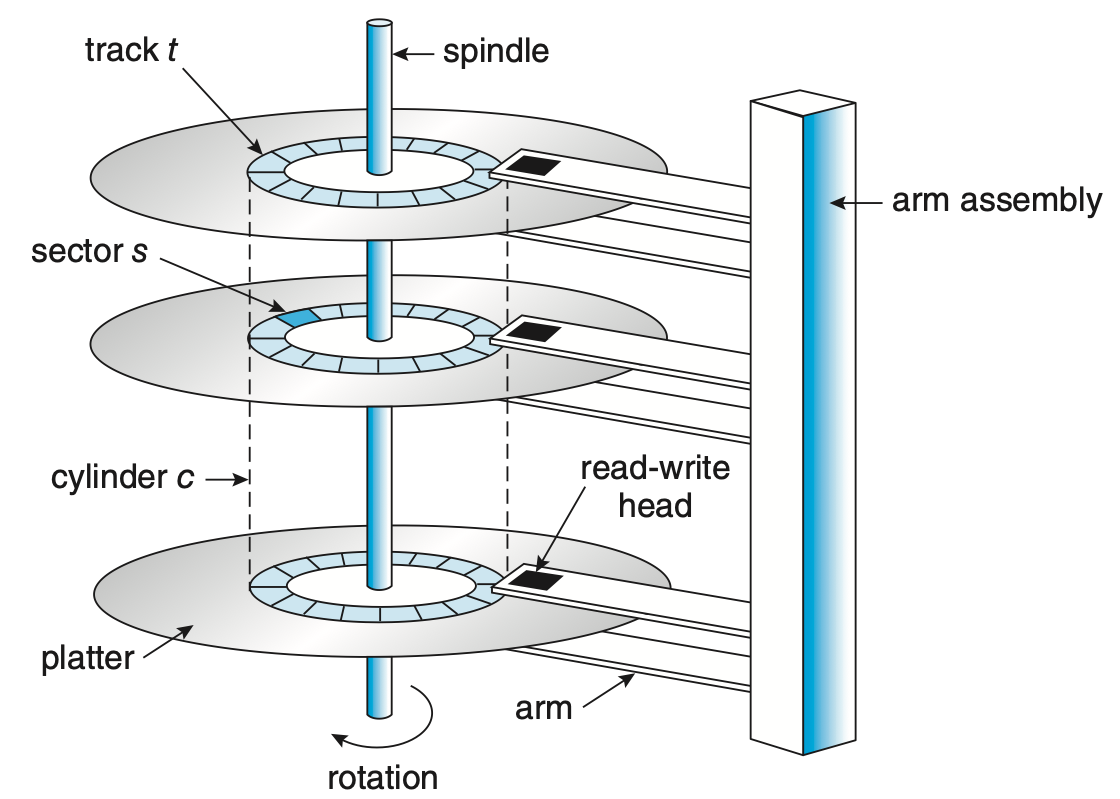
\includegraphics[width=0.618\linewidth]{pic/OS-CheatSheet/硬盘}
    \caption{Moving-head Disk Machanism}
\end{figure}

从硬盘上读写内容的过程如下:
\begin{enumerate}
    \item 磁头移动到指定的柱面;
    \item 磁头移动到指定的磁道;
    \item 磁盘旋转到扇区位于磁头下方;
    \item 读写扇区内容;
\end{enumerate}

disk 的平均 I/O 操作时间为: 
{\small
\begin{align*}
    \text{Average I/O time} 
    &= \underbrace{\text{average seek time} + \text{rotational latency}}_\text{average access time} \\
    &+ \underbrace{\frac{\text{data to transfer}}{\text{transfer rate}}}_{\text{transfer time}} \\
    &+ \text{controller overhead}
\end{align*}
}
\begin{itemize}
    \item 寻道时间(seek time):磁头移动到指定柱面的时间
    \item 旋转时延(rotational latency):目标扇区旋转到磁头下方的时间
    \subitem 一般以 round per minute(rpm) 表示,容易得到,平均旋转时延为 $\frac{1}{2}\frac{1}{rpm}60$s
    \item 传输时间(transfer time):数据在 disk 和 memory 之间传输的时间, 一般就是磁头扫过数据区域的时间. 
\end{itemize}

\paragraph{调度}加速 access time. 

disk bandwidth = 传输数据量 / 请求开始到传输完成的时间间隔

logical block address(LBA), logical block 是数据传输的最小单元

常见算法:
\begin{itemize}
    \item FCFS 
    \item SSTF (shortest seek time first)选择距离当前磁头最近的请求
    \item SCAN 算法下磁头在碰到 LBA 边界前只会单向移动,而在移动过程中处理能够处理的请求。
    \item LOOK 就是不走到底,而是走到最靠近边界的请求对应的 LBA 就提前掉头的SCAN. 
    \item C-SCAN 即 Circular SCAN,其磁头移动是始终单向的,当磁头达到 LBA 的边界时,径直返回到另一端,回程中不响应任何请求. 
    \item C-LOOK是在处理完最靠近边界的请求后就直接返回的C-SCAN. 
\end{itemize}

根据不同的应用场景选择不同的算法, 通常,SSTF 是比较常见的默认选择;而当 I/O 较为频繁的时候,一般使用 LOOK 或者 C-LOOK. 

\subsubsection{存储介质管理}
\begin{itemize}
    \item 分区(partitioning):将设备的存储空间做划分,每一个都被视为一个单独的存储空间(即一个 logical disk)。分区信息会以固定的格式被写入存储设备的固定位置。
    \item 卷创建与卷管理(volume creating \& management):卷(volume)是包含一个文件系统(file system)的存储空间,划定文件系统所覆盖的范围。如果直接在一个分区里安装文件系统,那其实这一步已经被隐式地完成;但如果使用比如 RAID 技术,就需要显示地做这一步。
    \item 逻辑格式化(logical formatting):在卷上创建和初始化文件系统。
\end{itemize}
同时,如果当前分区包含 OS 镜像,则需要对应初始化引导块(boot sector)。


\paragraph{RAID}0:无冗余 1:镜像 2:纠错码 3:奇偶校验 1个盘 4:按块条带化 Striping 5:校验盘分散到各个盘 6:P+Q 冗余,差错纠正码